\section{Benchmarks}
\label{sec:benchmark}

\subsection{Experiment system}
\label{sec:system}

In this section, we describe Mira - an IBM Glue Gene Q supercomputer in which we developed our algorithms and a framework for network load balancing and conducted our experiments. Mira \cite{Chen:BGQ}, with 48 compute racks (48K nodes and 768K cores) at the ALCF, provides 10 PFlops theoretical peak performance. Each node has a 16-core processor and 16 GB of memory.

The interprocess communications of Blue Gene/Q travel on a 5D torus network both for point-to-point and for collective communications. This 5D torus interconnects a compute node with its 10 neighbors at 2 GB/s theoretical peak over each link in each direction, making a total of 40 GB/s bandwidth in both directions for a single compute node. Because of packet and protocol overheads, however, only up to 90\% of the raw data rate (1.8 GB/s) is available for user data. The machine can be partitioned into non-overlapping rectangular submachines; these submachines do not interfere with each other except for I/O nodes and the corresponding storage system.

For interconnect network traffic, BG/Q supports both deterministic and dynamic routing \cite{Chen:BGQ}. In deterministic routing, packets are routed based on dimension-ordered routing, from the longest first to the shortest last. In dynamic routing, routing is still dimension-ordered, but it is programmable, enabling different routing algorithms to be used. Given the size of a certain message, routing is always the same, and its path is known before it is routed. These are the default routing algorithms and cannot be changed during run time. However, one can set which routing zone id to use by using the PAMI\_ROUTING environment variable. Since BG/Q uses single-path data routing, for sending/receiving a message only one link of the ten available is used. The details of routing can be found in \cite{Chen:BGQ}.

PAMI is a low-level communication library for BG/Q \cite{PAMI:Kumar}. PAMI provides low-overhead communication by using various techniques such as accelerating communication using threads, scalable atomic primitives, and lockless algorithms to increase the messaging rate. Since MPI is implemented on top of PAMI, direct use of PAMI would provide higher messaging rates as well as lower latencies in comparison with MPI.




\subsection{Experiment setup}

We carried our experiments on Mira, a Blue Gene/Q supercomputer. In our experiments, we varied paritition size from 512 nodes up to 8012 nodes. The experiments involved a subset or entire set of nodes for each partition. The number sources and destinations and distance between them are also varied depending on each experiment. We also varied the data sizes to be exchanged to find the effective data size. Pairs of sources and destinations are randomized to show the efficacy of our works. We varied the number of paths fed into solvers to measure the effectiveness of number of paths to throughput. A similar benchmark with various max load is done for heuristic approach. Our experiments covered 3 communication patterns: Disjoint, Overlap and Subset. For the commnication patterns, we demonstrated the efficacy of our algorithms in comparions with MPI\_Alltoallv.

For searching optimal paths, we used AMPL (A Modeling Language for Mathematical Programming) and its solvers \cite{AMPL} for modeling our problem and to find solutions for optimal data movement.


%%\subsection{MPI path reconstruction}

We measure several network-related metrics such as load on physical links, and the number of hops per data-transfer path, for the above benchmarks, using our approaches and MPI\_Alltoallv. The load and number of hops highlight performance differences between MPI and OPTIQ. The performance metrics are output directly in case of OPTIQ. However, MPI\_Alltoallv does not output all of these performance metrics. Thus, we need to reconstruct the data-transfer paths taken by MPI collectives. We reconstruct the paths based on the routing algorithms described in \cite{Chen:BGQ}. For each pair of source and destination nodes, we start at a source node and trace the route taken by the MPI message according to the rules of the routing algorithm. We record paths for all source-destination pairs and use this information to calculate load and number of hops for MPI\_Alltoallv. 

%In our experiment we need to measure not only the performance of MPI routines, but also loads on physical links, and the number of hops per path that MPI takes to move data from a set of sources to a set of destination. The load and hops information can reveal details on performance differences between MPI and our framework OPTIQ. Thus reconstructing MPI's paths is necessary to get load and hops information.
%We reconstruct MPI's paths based on our understanding of default routing algorithms described in \cite{Chen:BGQ}. For each pair of source and destination we start at a source node and follow the rules of the routing algorithm to move data from the source node to its destination. We then record paths for all the pairs and use them to calculate load and number of hops.


We demonstrate the data movement performance of our OPTIQ framework and existing MPI routines on three communication patterns -- {\em disjoint}, {\em overlap} and {\em subset}, illustrated in Figure \ref{fig:patterns}. In this figure, m and n refer to set of source or destination nodes. These patterns are owing to different possible relationships between source and destination nodes as described below:
\begin{itemize}
\item Disjoint: There are distinct sources and destinations. It is a common data movement pattern present in many applications.
\item Overlap: The sources and destinations are overlapped sets. Some applications like CESM uses this communication pattern for coupling.
\item Subset: Either the set of source nodes is subset of the destination nodes or vice versa. This pattern can be found in CESM and in collective I/O aggregation phase.
\end{itemize}
\begin{figure}[ht]
\vspace{-0.15in}
\centering
\includegraphics[scale=0.48]{figures/patterns.pdf}
\vspace{-0.15in}
\caption{\small Communication patterns}
\vspace{-0.15in}
\label{fig:patterns}
\end{figure}

We demonstrate throughput improvement in a complex network like 5D torus through the above diverse communication patterns. We compare the efficacy of our algorithms with MPI\_Alltoallv, which is the most commonly used MPI collective for the data movement patterns considered in our work.


\subsection{Experiments and Results}

We carried out a set of experiments in which we varied total number of nodes, number of sources, number of destinations, distance between source nodes and destination nodes. We measured the follows: throughput of data transfer, total number of paths found, number of paths per pair of source-destination (a job), hopbytes (multiplication of an amount of data and a number of hops it travels on a path) values on a path, number of paths that shares a physical link, and amount data that passes through a physical link. We used our framework OPTIQ and MPI\_Alltoallv to transfer data and compare 2 ways to show the efficacy of our framework. MPI\_Alltoallv is typical way to transfer data between a set of sources and a set of destinations. It uses default routing algorithms i.e. both dynamic and static routing can be employed.

\subsubsection{Varying partition, source and destination sizes, keeping the same source to destination ratio}

In this experiment we vary the number of sources and destinations, together with total number of nodes, while keeping a constant ratio of 1:8 between the number of sources and destination nodes. We increase the total number of nodes P from 512 to 4096, The first P/16 nodes send data to the last P/2 nodes. Each source has 8 destinations e.g. node 0 sends data to nodes P/2, P/2+1, ... P/2+7. We present results for {\em disjoint}, {\em overlap} and {\em subset} communications using OPTIQ Optimization (OPT), OPTIQ Heuristic (HEU) and MPI\_Alltoallv (MPI). We use 1 MPI/PAMI rank/node. The data size is 8 MB per source-destination pair. 
%We set the $maxload$ to 16 for the Heuristic approach. %already mentioned 

Figure \ref{fig:constantr} shows the throughput for OPT, HEU and MPI. As shown in the figure, the Optimization approach has the highest throughput, followed by the Heuristic approach and MPI\_Alltoallv. This is because OPT and HEU uses multiple paths for data transfer. Additionally, OPT globally balances load for all source-destination pairs. %TODO: We see improved throughput for 4096 nodes in the case of OPT and HEU because ..... data / hopbytes for 512 vs 4096 performance.  

\begin{figure*}[!htbp]
        \centering
        \begin{subfigure}[b]{0.32\textwidth}
                \includegraphics[width=\textwidth]{figures/constantr_3.pdf}
                \caption{Disjoint}
                \label{fig:constantr_3}
        \end{subfigure}%
        ~ %add desired spacing between images, e. g. ~, \quad, \qquad, \hfill etc.
          %(or a blank line to force the subfigure onto a new line)
        \begin{subfigure}[b]{0.32\textwidth}
                \includegraphics[width=\textwidth]{figures/constantr_27}
                \caption{Overlap}
                \label{fig:constantr_27}
        \end{subfigure}
        ~ %add desired spacing between images, e. g. ~, \quad, \qquad, \hfill etc.
          %(or a blank line to force the subfigure onto a new line)
        \begin{subfigure}[b]{0.32\textwidth}
                \includegraphics[width=\textwidth]{figures/constantr_87}
                \caption{Subset}
                \label{fig:constantr_87}
        \end{subfigure}
        \caption{\small Varying the number of sources and destinations and total number of nodes while keeping the ratio constant (1:8).}
	\vspace{-0.15in}
        \label{fig:constantr}
\end{figure*}

Table \ref{table:constantr} shows the throughput, total number of paths per job, the hopbytes per path, the number of copies per path, number of paths per physical link and the total data per link for 1024 nodes. In all three cases, our greedy heuristic is able to find the highest number of paths for the entire data flow. HEU also has the highest maximum and average number of paths per job. However, the paths found by Heuristic are based on local optimization of load on the physical links, as explained in Section~\ref{sec:heuristic}. Therefore, there are higher number of paths per physical link, and higher amount of data per physical link in HEU as compared to OPT. OPT has lower number of paths per link because OPT globally load balances the data transfer on physical links.
%TODO: table remove columns
\begin{comment}
\begin{table*}[!htbp]
   \centering
    \begin{tabular}{| p{0.5cm} | l | r | r | p{0.5cm} | p{0.5cm} | p{0.5cm} | p{0.5cm} |p{0.4cm} | p{0.5cm} |p{0.4cm} | p{0.4cm} |p{0.50cm} | p{0.6cm} |}
    \hline
    \multirow{3}{*}{Pattern} & \multirow{3}{*}{Type} & \multirow{3}{1cm}{nW (GB/s)} & \multicolumn{3}{ c| }{Num. of Paths} & \multicolumn{2}{ c| }{Hopbytes} & \multicolumn{2}{ c| }{Num of copies}& \multicolumn{2}{ c| }{Num of paths} & \multicolumn{2}{ c| }{Total data} \\ \cline{4-6}
    & & & \multirow{2}{0.5cm}{Total Paths} & \multicolumn{2}{ c| }{Per Job} & \multicolumn{2}{ c| }{Per Path (MB)} & \multicolumn{2}{ c| }{Per Path}& \multicolumn{2}{ c| }{Per Link}& \multicolumn{2}{ c| }{Per Link (MB)} \\ \cline{5-14}
    & & & & {Max} & Avg & Max & Avg & Max & Avg & Max & Avg & Max & Avg\\ \hline
    \multirow{3}{*}{Disjoint} & OPT    & 188.62 & 1169 & 6 & 2.28 & 83.88 & 23.02 & 1152 & 295.22 & 11 & 2.53 & 18.28 & 9.26 \\ \cline{2-14}
    & HEU & 74.88  & 3146 & 23 & 6.14 & 83.88 & 8.45 & 1152 & 108.24 & 16 & 4.94 & 63.04 & 6.92 \\ \cline{2-14}
    & MPI    & 45.18  & 512  & 1 & 1.00 & 92.27 & 50.33 & & & 16 & 3.07 & 134.21 & 25.76\\ \hline
    \multirow{3}{*}{Overlap} & OPT    & 200.03 & 1303 & 6 & 2.54 & 83.88 & 19.28  & 1152 & 243.96 & 13 & 2.74 & 16.97 & 9.04\\ \cline{2-14}
    & HEU & 113.17  & 3273 & 26 & 6.39 & 75.49 & 7.41 & 1024 & 93.07 & 16 & 5.17 & 38.66 & 7.04 \\ \cline{2-14}
    & MPI    & 42.84 & 512 & 1 & 1.00 & 83.88 & 42.99 &  & & 16 & 3.38 & 134.21 & 28.36 \\ \hline
    \multirow{3}{*}{Subset} & OPT    & 199.20 & 1269 & 6 & 2.48 & 75.49 & 19.48 & 1024 & 245.66 & 11 & 2.79 & 17.10 & 9.32 \\ \cline{2-14}
    & HEU &  61.71 & 3238 & 26 & 6.32 & 75.49 & 7.43 & 1024 & 93.22 & 16 & 5.28 & 45.08  & 7.35 \\ \cline{2-14}
    & MPI    &  41.37 & 512  & 1 & 1.00 & 83.88 &  41.94 & & & 16 & 3.52 & 134.21 & 29.49 \\ \hline
    \end{tabular}
    \caption{\small Throughput, total number of paths, number of paths per job, maximum and average values of hopbytes, number of copies, number of paths per link and amount of data per link for 3 patterns in 1024 nodes experiments.}
    \label{table:constantr}
\end{table*}
\end{comment}

\begin{table}[!htbp]
   \centering
    \begin{tabular}{| L{0.65cm} | L{0.4cm} | R{0.6cm} | R{0.5cm} | R{0.3cm} | R{0.4cm} | R{0.4cm} | R{0.3cm} | R{0.90cm} |}
    \hline
    \multirow{3}{*}{Pattern} & \multirow{3}{*}{Type} & \multirow{3}{0.6cm}{BW (GB/s)} & \multicolumn{3}{ c| }{Num. of Paths} & \multicolumn{2}{ c| }{Num of paths} & \multirow{3}{1.15cm}{Max amt. of data / link (MB)} \\ \cline{4-6}
    & & & \multirow{2}{0.5cm}{Total Paths} & \multicolumn{2}{ c| }{Per Job} & \multicolumn{2}{ c| }{Per Link}& \\ \cline{5-8}
    & & & & {Max} & Avg & Max & Avg & \\ \hline
    \multirow{3}{*}{Disjoint} & OPT    & 188.62 & 1169 & 6 & 2.28 & 11 & 2.53 & 18.28 \\ \cline{2-9}
    & HEU & 74.88  & 3146 & 23 & 6.14 & 16 & 4.94 & 63.04 \\ \cline{2-9}
    & MPI    & 45.18  & 512  & 1 & 1.00 & 16 & 3.07 & 134.21 \\ \hline
    \multirow{3}{*}{Overlap} & OPT    & 200.03 & 1303 & 6 & 2.54 & 13 & 2.74 & 16.97 \\ \cline{2-9}
    & HEU & 113.17  & 3273 & 26 & 6.39 & 16 & 5.17 & 38.66 \\ \cline{2-9}
    & MPI    & 42.84 & 512 & 1 & 1.00 & 16 & 3.38 & 134.21 \\ \hline
    \multirow{3}{*}{Subset} & OPT    & 199.20 & 1269 & 6 & 2.48 & 11 & 2.79 & 17.10 \\ \cline{2-9}
    & HEU &  61.71 & 3238 & 26 & 6.32 & 16 & 5.28 & 45.08 \\ \cline{2-9}
    & MPI    &  41.37 & 512  & 1 & 1.00 & 16 & 3.52 & 134.21 \\ \hline
    \end{tabular}
    \caption{\small Throughput, total number of paths, number of paths per job, maximum and average values number of paths per link and max amount of data per link for 3 patterns in 1024 nodes experiments.}
    \vspace{-0.15in}
    \label{table:constantr}
\end{table}

Figure \ref{fig:loaddata_histo} shows the distribution of data per link for OPT, HEU and MPI. Optimization approach considers the global load on the network and hence data is distributed among the paths in a more balanced way such that the physical links are load-balanced. Thus, OPT has the lowest maximum amount of data per physical link as shown in Figure \ref{fig:loaddata_histo}. MPI\_Alltoallv has the lowest number of paths. With 1 path per pair of communication, entire data is transferred using the single path, without utilizing the other idle links. %Thus it has the highest hopbytes per path as can be observed in Figure \ref{fig:hopbyte_histo}. 
MPI has the highest amount of data per physical link as can be observed in Figure \ref{fig:loaddata_histo}. Thus MPI has the lowest throughput.
\begin{figure}[!htb]
\vspace{-0.15in}
\centering
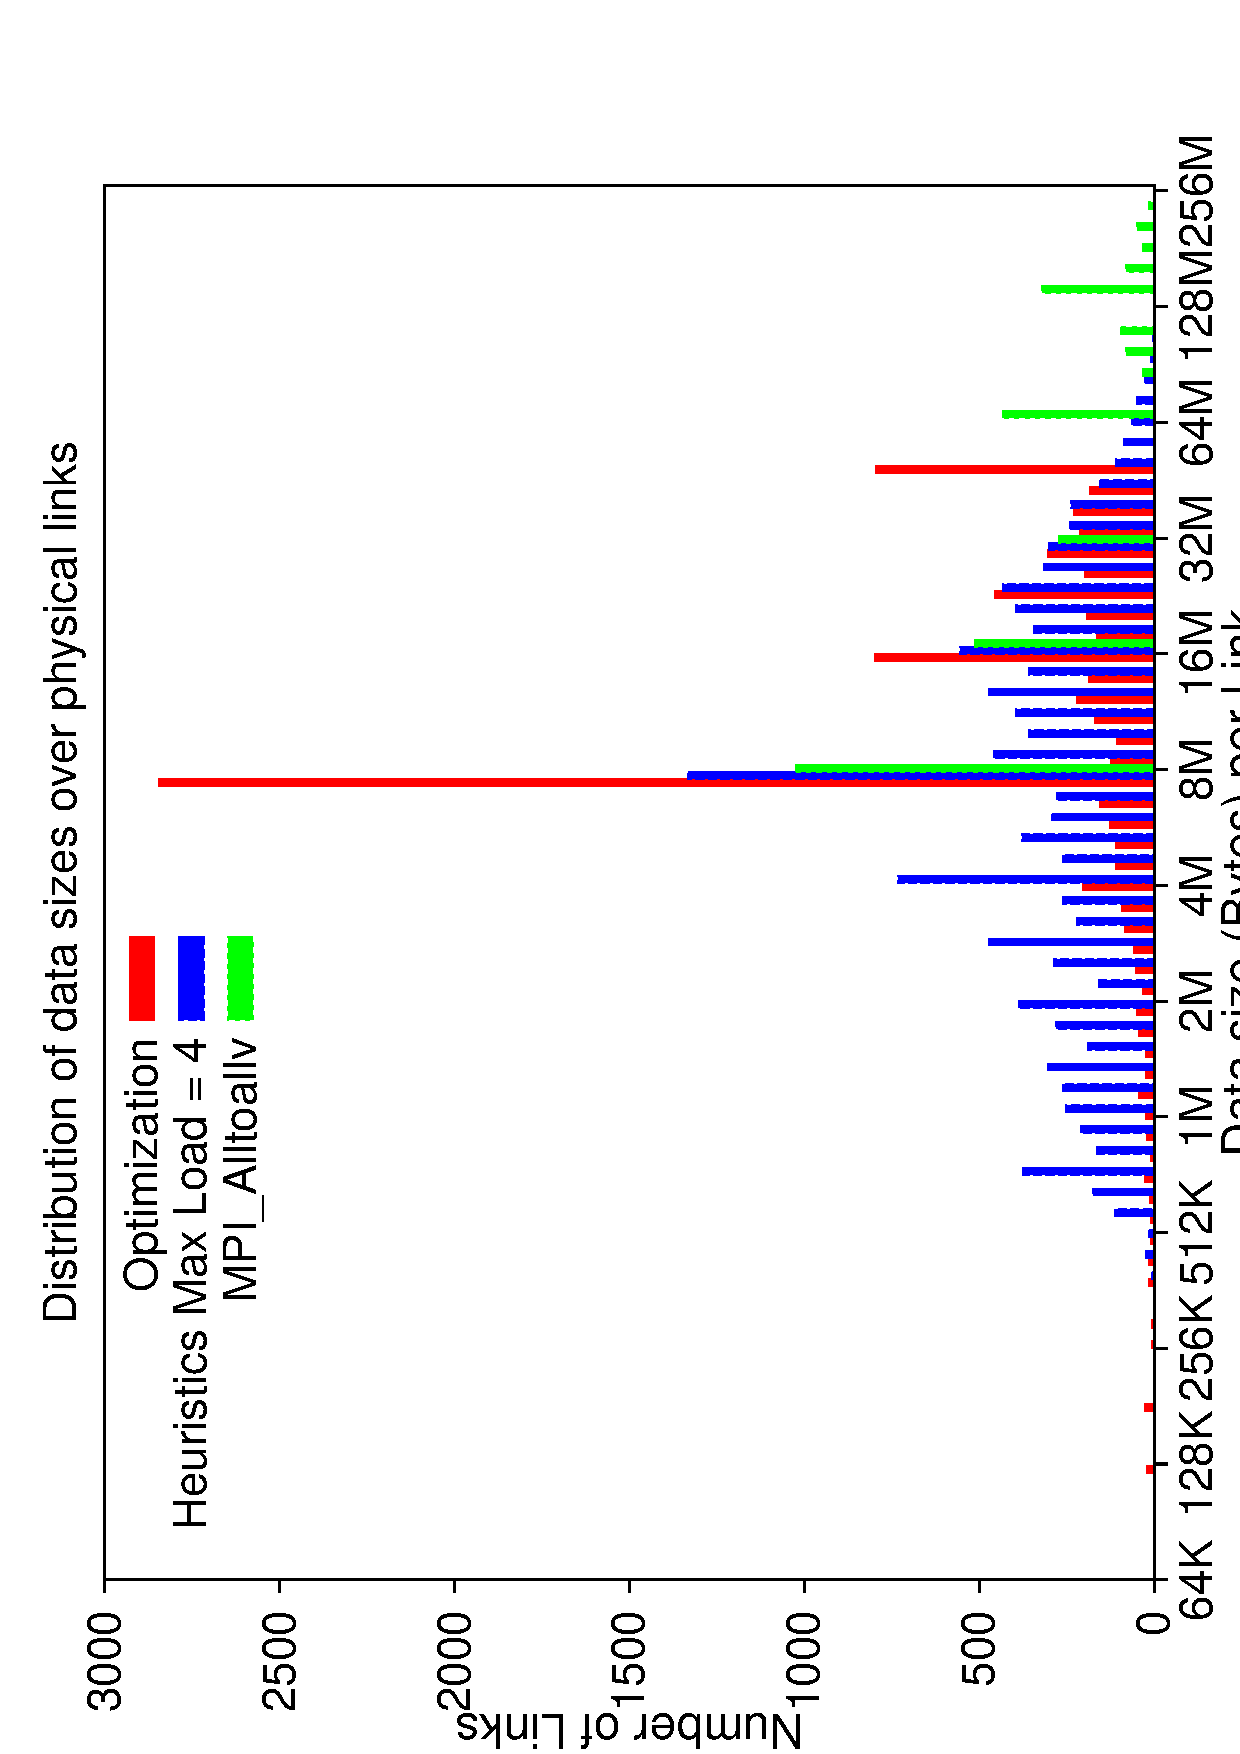
\includegraphics[scale=0.27]{figures/loaddata_histo.pdf}
\vspace{-0.15in}
\caption{\small Distribution of total amount of data per link for Disjoint pattern in 1024-node partition.}
\vspace{-0.15in}
\label{fig:loaddata_histo}
\end{figure}

%\begin{figure}[!htb]
%\vspace{-0.1in}
%\centering
%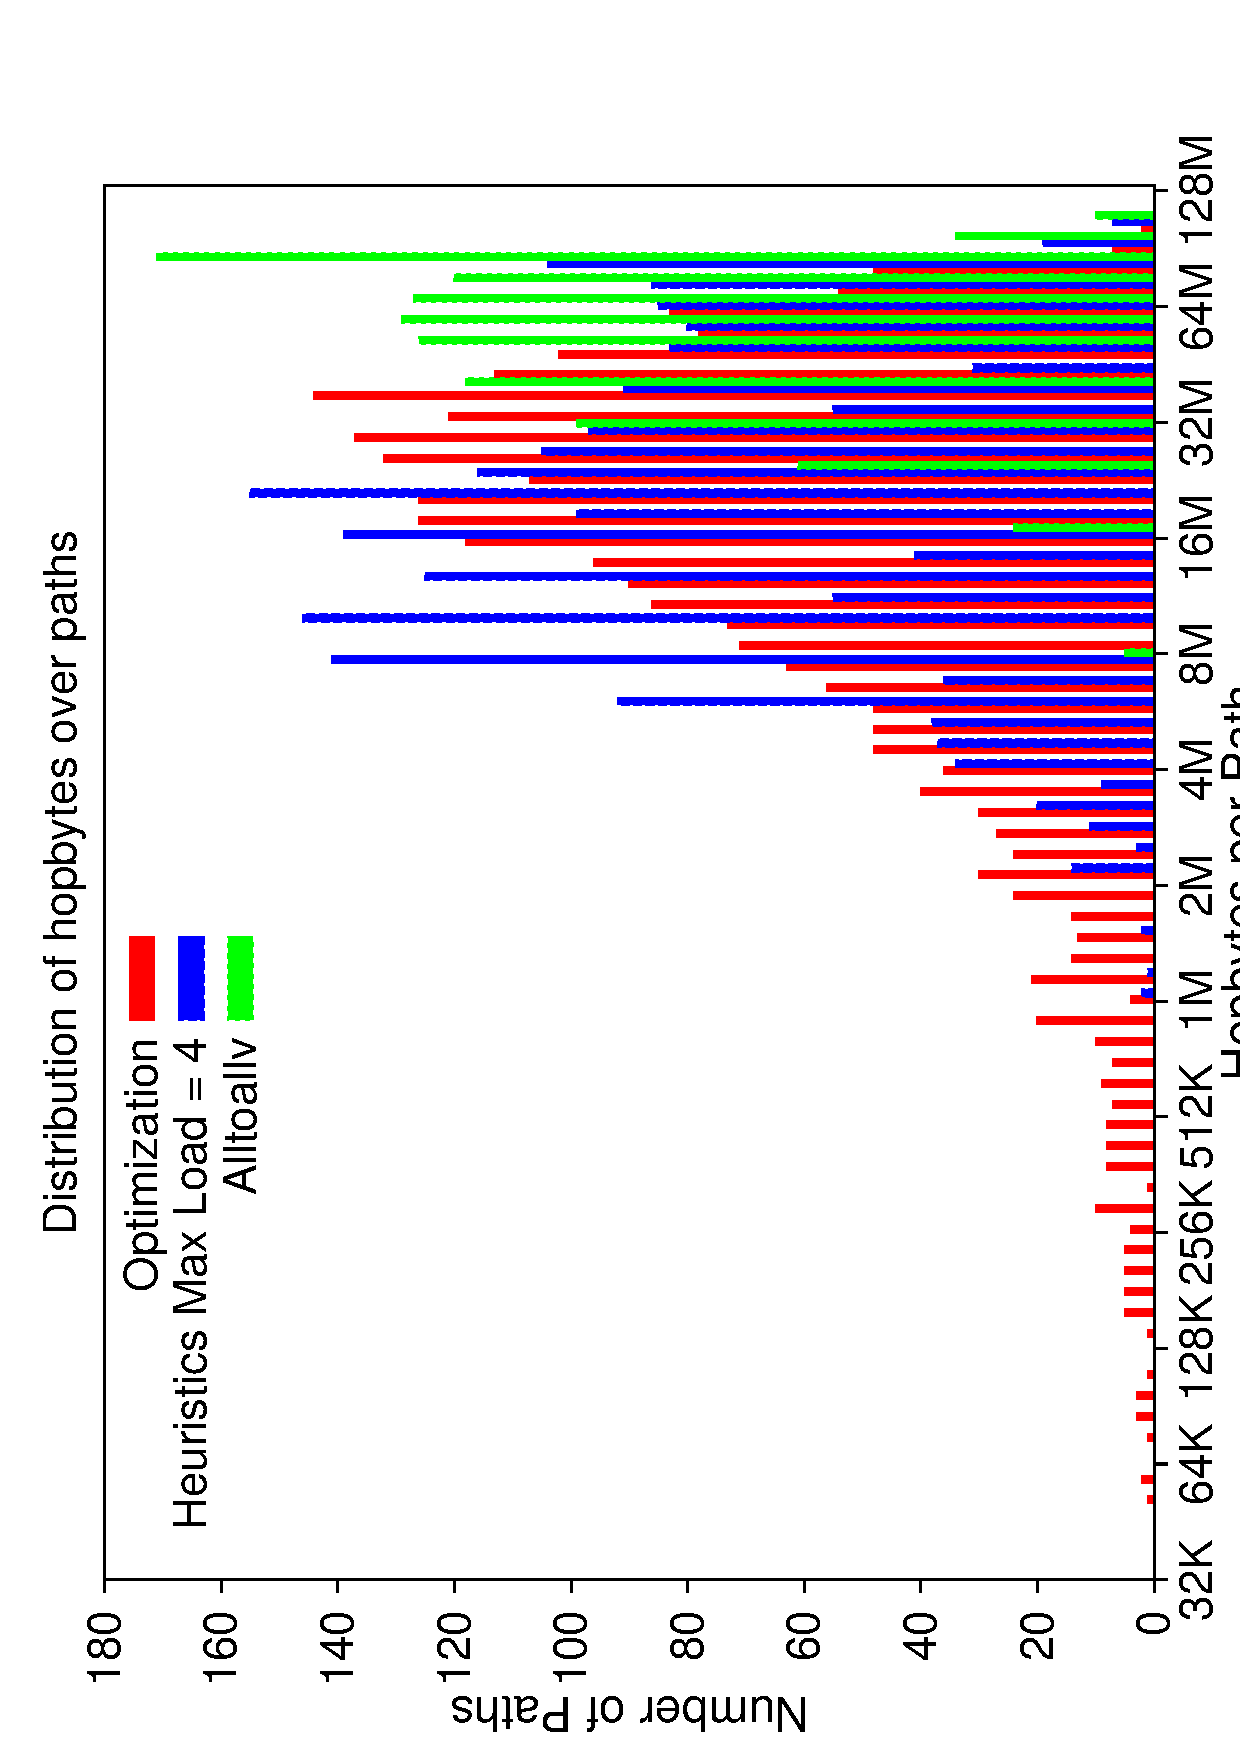
\includegraphics[scale=0.30]{figures/hopbyte_histo.pdf}
%\vspace{-0.1in}
%\caption{Distribution of hopbytes per path for Disjoint pattern in 1024-node partition.}
%\vspace{-0.1in}
%\label{fig:hopbyte_histo}
%\end{figure}




\subsubsection {Three communication patterns with random message sizes}
In this experiment, we varied the message sizes.


%\subsubsection {Multiple ranks}
%In this experiment, we demonstrate the scalabity of our framework when increasing the number of MPI/PAMI ranks per node.

